% =====================================================================
%  Chapter 24 — The Stated Policy and Its Justification
% =====================================================================

\chapter{The Stated Policy and Its Justification}
\label{ch:policy}

The policy is 36 per cent United States equity, 24 per cent equity outside
the United States, 30 per cent bonds\idx{Bonds}, and 10 per cent real assets. This
chapter argues for those numbers, states what the argument does not cover,
and reports what the record looks like under two alternatives.

\section{The arithmetic of the policy}

The 60/30/10 split between growth assets, bonds and real assets\idx{Real assets} is a
house view, and the book is explicit that it is one. What can be argued
is the internal consistency of the split and the choice of the equity
split inside the growth half.

\begin{equation}
\underbrace{0.60}_{\text{growth: } 0.36 + 0.24}
\;+\;
\underbrace{0.30}_{\text{bonds}}
\;+\;
\underbrace{0.10}_{\text{real assets}}
\;=\; 1.
\end{equation}

The sixty per cent growth allocation is the conventional anchor for a
long-horizon investor, and it is not defended here on the grounds that it
maximises expected return --- Chapter 3's evidence says that
expected-return estimates are the least reliable thing in the literature.
It is defended on the grounds that it is the allocation a saver can
actually hold, and that the book's risk layer is designed to reduce the
drawdown that a sixty per cent growth allocation produces.

The bond allocation is thirty per cent, split between Treasuries, aggregate
bonds, credit and inflation-protected bonds inside the sleeve. It is
large enough to matter in an equity-led drawdown and small enough that the
investor is not running a balanced portfolio with an equity overlay.

The real-asset allocation is ten per cent, spread across gold, real
estate and broad commodities. This is the smallest of the four and the
one with the weakest individual case: Chapter 22's regime argument
applies to commodities in particular, and a portfolio that depends on
commodities for its diversification\idx{Diversification} is depending on a regime. Ten per cent
is small enough that being wrong about it is not catastrophic.

Inside the growth half, the split is 60 per cent United States and 40 per
cent non-United States, which is close to the world market capitalisation
weights of the period. That is the justification: the non-United States
allocation is there for the correlation and currency structure of the
international market, not for an expected-return premium, and the closest
approximation to a neutral weight for that purpose is the market's own.

\begin{figure}[!htbp]
\centering
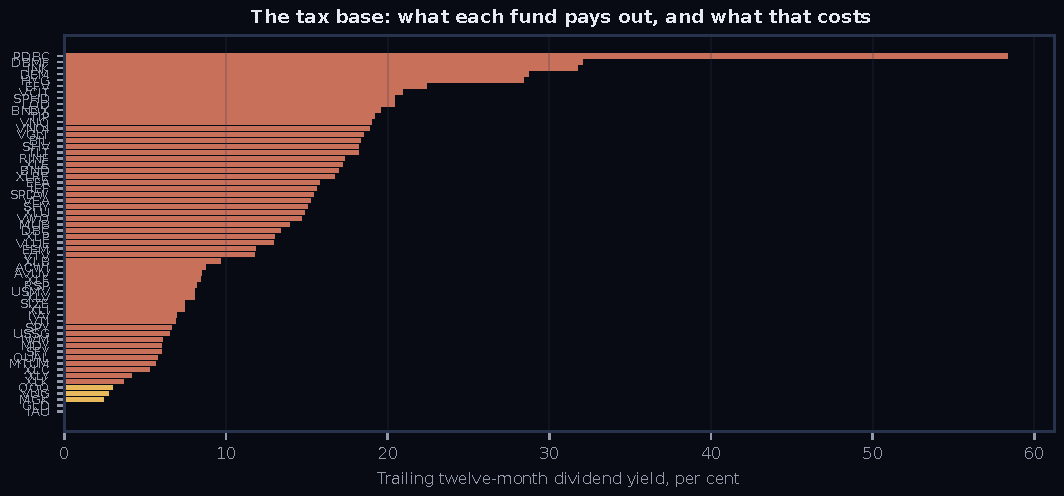
\includegraphics[width=\textwidth]{../figures/fig_yields.pdf}
\caption{The dividend yield of each sleeve's representative funds over the
record, and the yield the reader was paid for waiting. The yield is not a
premium in the risk-premium sense; it is compensation for taking the
duration and the credit risk, and it is what makes the bond sleeve a
participant in the compounding rather than a place to hide.}
\label{fig:yields}
\end{figure}

\section{What the argument does not cover}

Three exclusions, stated plainly.

It does not claim the policy is optimal. Nothing in this book can support
such a claim, and the evidence of Chapter 3 is that anyone who claims it
is probably overfitting.

It does not claim the policy is robust to every alternative. The book
reports the record under a defensive policy of 24/16/30/30 and an
aggressive one of 48/32/15/5, in Chapter 33, so that the reader can see
the spread.

It does not claim the policy is the right one for every reader. It is
the policy for a reader with a long horizon, a stable income and an
ability to sit through a thirty per cent drawdown. A reader who cannot
sit through that should change the policy, and Chapter 38 says how.

\section{Why the policy is stated rather than derived}

The obvious alternative --- derive the allocation from the data by
optimising some objective over the historical record --- is the one the
literature does, and Chapter 3's evidence says what happens to it.

Consider what such a derivation would involve. The objective would be
some function of the historical returns; the parameters would be chosen
by some rule; and the result would be an allocation that is optimal on
the data that produced it. There is no way to distinguish such an
allocation from one that is overfitted, except by the size of the
improvement --- and the improvement is measured on the same data that
selected it.

The stated policy has the opposite property. It cannot be overfitted,
because it was not fitted. It can be wrong, and it is quite likely to be
wrong in the sense that a different fixed allocation might have done
better over this particular record --- but being wrong in that way is
harmless, because the reader never chose it on the basis of the record.
The reader chose it on the basis of an argument, and they can evaluate the
argument.

\begin{takeaway}[Why stated, not derived]
A derived allocation is optimal on the data that selected it, and there is
no way to tell it from an overfitted one except by the size of its
apparent improvement on the same data. A stated allocation can be wrong;
what it cannot be is overfitted, because it was never fitted. The reader's
decision is an argument, not a fit.
\end{takeaway}

\section{The alternatives the book runs}

Because a stated policy is a claim, the book tests it against two
alternatives that are also stated, and the three are all in the trial
family so that the selection machinery sees them.

\textbf{The defensive policy:} 24 per cent United States equity, 16 per
cent international, 30 per cent bonds, 30 per cent real assets. This is a
retiree drawing down.

\textbf{The aggressive policy:} 48 per cent United States equity, 32 per
cent international, 15 per cent bonds, 5 per cent real assets. This is a
young saver with a long horizon and a tolerance for a fifty per cent
drawdown.

The book does not claim to know which is best. It reports all three, with
their drawdowns and their recoveries, and lets the reader read the
trade-off: the aggressive policy earns more over this record and gives up
six percentage points of drawdown, and the defensive policy earns less and
sits through a shallower episode.

\begin{keytakeaways}
\item The 60/30/10 split is a house view, defended for internal
consistency and for the reader's ability to hold it, not for optimality.
\item The 60:40 United States to non-United States split inside the growth
half is justified by market capitalisation as the closest neutral weight
for the diversification and currency argument.
\item A stated policy cannot be overfitted because it was never fitted;
that is the whole reason for stating it.
\item Two alternative policies are stated and run, so the reader can see
the growth against the drawdown trade-off rather than being handed one
number.
\end{keytakeaways}
